% \VignetteIndexEntry{shinyMethyl: interactive visualization of Illumina 450K methylation arrays}
% \VignettePackage{shinyMethyl}
% \VignetteDepends{BiocStyle}
% \VignetteEngine{knitr::knitr}

\documentclass[12pt]{article}
\usepackage[numbers]{natbib}
\usepackage{amsthm}
\newcommand{\minfi}{\Biocpkg{minfi}}

\RequirePackage{/Library/Frameworks/R.framework/Versions/3.1/Resources/library/BiocStyle/sty/Bioconductor}

\AtBeginDocument{\bibliographystyle{/Library/Frameworks/R.framework/Versions/3.1/Resources/library/BiocStyle/sty/unsrturl}}


\title{Functional normalization: reproducible report}
\author{Jean-Philippe Fortin, Kasper Daniel Hansen}
\begin{document}

\maketitle{}
\setcounter{secnumdepth}{1} 

% Introduction
\section{Introduction}

 \url{https://github.com/Jfortin1/funnorm_repro}

\begin{knitrout}
\definecolor{shadecolor}{rgb}{0.969, 0.969, 0.969}\color{fgcolor}\begin{kframe}
\begin{alltt}
\hlstd{funnormDir} \hlkwb{<-} \hlstr{"/Users/Jean-Philippe/funnorm_repro"}
\hlkwd{setwd}\hlstd{(}\hlstr{"/Users/Jean-Philippe/funnorm_repro/"}\hlstd{)}
\end{alltt}
\end{kframe}
\end{knitrout}

\subsection{Scripts directory}
\subsection{Cluster jobs file}

The shell script \Rcode{jobs.sh} contain all the ordered jobs that were submitted to the cluster. 

\subsection{Extraction of the data}
\subsection{Metadata}
The folder \Rcode{/metadata} contains the mappings file from TCGA for the AML and KIRC datasets, for both 27k and 450k platforms. These \Rcode{.csv} files contain the names of the samples, the plate information, sample tissue and histology of the samples (used as the phenotype for the subsequent analysis). 

The file \Rcode{clinical\_patient\_laml-1.txt} contains the clinical leukemia tumor subtype defined by \fixme{FAB}. 

The file \Rcode{link27kto450k.Rda} pairs the AML 27k samples to their corresponding 450k samples.


\subsection{Experimental designs}

The folder \Rcode{/designs} contain all the design information to construct the discovery and validation datasets used throughout the analysis. For instance, for the KIRC dataset, the design file is called \Rcode{design\_kirc.Rda} and contains the sample names, the phenotypic group and the discovery/validation set identification as follows:

\begin{knitrout}
\definecolor{shadecolor}{rgb}{0.969, 0.969, 0.969}\color{fgcolor}\begin{kframe}
\begin{alltt}
\hlkwd{setwd}\hlstd{(}\hlkwd{file.path}\hlstd{(funnormDir,} \hlstr{"designs"}\hlstd{))}
\hlkwd{load}\hlstd{(}\hlstr{"design_kirc.Rda"}\hlstd{)}
\hlkwd{head}\hlstd{(design_kirc)}
\end{alltt}
\begin{verbatim}
##                          sampleName group        set
## 6042316009_R02C02 6042316009_R02C02 Tumor Validation
## 6042316009_R03C01 6042316009_R03C01 Tumor Validation
## 6042316009_R04C01 6042316009_R04C01 Tumor Validation
## 6042316009_R04C02 6042316009_R04C02 Tumor Validation
## 6042316009_R06C01 6042316009_R06C01 Tumor Validation
## 6042316009_R06C02 6042316009_R06C02 Tumor Validation
\end{verbatim}
\end{kframe}
\end{knitrout}


The file \Rcode{create.design.aml.R} extracts the AML tumor subtype from the file \Rcode{clinical\_patient\_laml-1.txt} for the AML samples. 

\subsection{Plate information}

The directory \Rcode{/plate\_info} contains the physical plate information of the samples for each dataset. This information is used in the ComBat method [[]] and in the plate adjustment model used for the 27k data. 

\begin{knitrout}
\definecolor{shadecolor}{rgb}{0.969, 0.969, 0.969}\color{fgcolor}\begin{kframe}
\begin{alltt}
\hlkwd{setwd}\hlstd{(}\hlkwd{file.path}\hlstd{(funnormDir,}\hlstr{"plate_info"}\hlstd{))}
\hlkwd{load}\hlstd{(}\hlstr{"kirc_plate_450k.Rda"}\hlstd{)}
\hlkwd{head}\hlstd{(kirc_plate_450k)}
\end{alltt}
\begin{verbatim}
##                          sampleName plate
## 6042324009_R01C01 6042324009_R01C01    90
## 6042324009_R02C01 6042324009_R02C01    90
## 6042324009_R04C01 6042324009_R04C01    90
## 6042324009_R05C01 6042324009_R05C01    90
## 6042324009_R02C02 6042324009_R02C02    90
## 6042324009_R03C02 6042324009_R03C02    90
\end{verbatim}
\end{kframe}
\end{knitrout}

The companion script \Rcode{create.plate.info.R} was used to extract the physical plate information of the samples. 

\subsection{Loading the data in \R}

For each dataset, we read the data into \R{} using the packages \Biocpkg{minfi} and \Biocpkg{methylumi}. The first package produces an \Rcode{RGChannelSet} for each dataset, while the latter package produces a \Rcode{MethyLumiSet}. The reason why we use both packages to read the data is that the \textit{noob} normalization method is implemented in the \Biocpkg{methylumi} package, while all other normalization methods are compatible with \Biocpkg{minfi}. For each dataset, the files are saved in the \Rcode{/raw\_datasets} directory. For instance, \Rcode{rgset\_kirc.Rda} and \Rcode{methylumi\_kirc.Rda} correspond to the \Rcode{RGChannelSet} and \Rcode{methyLumiSet} for the KIRC dataset, respectively. 

\subsection{Production of the discovery and validation datasets}
The folder \Rcode{dis\_val\_datasets} contains the code to create the discovery and validation datasets objects. For instance, the script \Rcode{create.dis.val.methylumi.R} will produce the \Rcode{MethyLumiSet} object for each discovery and validation subsets of each datasets, and these objects will be saved in this directory under the name \Rcode{methylumi\_dis\_XXX} and \Rcode{methylumi\_val\_XXX} where XXX is the name of the dataset, for instance \textit{kirc}. 

\section{Normalization}

All the scripts to produce the normalized datasets can be found in the folder \Rcode{/norm\_datasets}. 

\subsection{Normalization for raw, funnorm, quantile, SWAN and dasen methods }
The file \Rcode{create.norm.R} is used to produce the normalized datasets for the raw, funnorm, quantile, SWAN and dasen methods. It will produce files of the form \Rcode{norm\_dis\_XXX.Rda} and \Rcode{norm\_val\_XXX.Rda} in the same directory that contains the normalized data. 

For example, the object stored in \Rcode{norm\_dis\_kirc.Rda} is a list of 5 matrices corresponding to the normalized Beta values for each aforementioned method, for the KIRC discovery dataset. 

\subsection{Normalization for noob method}

Since the \textit{noob} method requires a \Rcode{MethyLumiObject}, we use a different script to produce the normalized datasets. The script \Rcode{create.norm.noob.R} is used to produce these datasets, and the normalized datasets are saved under the name \Rcode{noob\_dis\_XXX.Rda} and \Rcode{noob\_val\_XXX.Rda}. 

\subsection{Normalization for funnorm + noob method}

The script \Rcode{create.funnorm.noob.R} generates the normalized data for the funnorm method that includes the background correction as implemented in the \Biocpkg{methylumi} (noob). The normalized data can be found in the files \Rcode{funnorm\_noob\_dis\_XXX.Rda} and \Rcode{funnorm\_noob\_val\_XXX.Rda}.

\subsection{Normalization for BMIQ}

Because BMIQ is extremely slow and no parallel method is implemented yet, the normalization of the data with BMIQ requires a special treatment. 

The script \Rcode{split.bmiq.R} will read in it \Rcode{RGChannelSet}, and will split the data into individual samples, and resave the samples separately in the folder \Rcode{/funnorm\_repro/raw\_datasets/all\_samples}. This folder contains the 1460 individual samples saved in \Rcode{.Rda files} (for instance, \Rcode{6042308157\_R06C01.Rda}). 

Since BMIQ does not perform between-array normalization, we can normalize all these samples in an embarrassingly parallel way; that's what the script \Rcode{create.norm.bmiq.R} does. It uses the version 1.3 of BMIQ that can be found in the \Rcode{/scripts} folder.

The normalized samples will be saved in the folder \Rcode{/funnorm\_dir/norm\_datasets/all\_samples\_bmiq}. 

The script \Rcode{merge.norm.bmiq.R} will merge back the normalized samples and will create the files \Rcode{bmiq\_dis\_XXX.Rda} and \Rcode{bmiq\_val\_XXX.Rda} for each dataset XXX. 

\subsection{Merging all the normalized data}

For each dataset, the script \Rcode{merge.all.norm.R} will merge all the normalized data above in files called \Rcode{all\_norm\_dis\_XXX.Rda} and \Rcode{all\_norm\_val\_XXX.Rda}. 

\section{Creation of the DMPs}

For each dataset, we create a list of differentially methylated positions (DMPs) with the corresponding dataset phenotype. The script \Rcode{create.dmps.R} located in the directory \Rcode{/dmps} is used to create those lists. For each dataset, the results are stored in files \Rcode{dmps\_dis\_XXX.Rda} and \Rcode{dmps\_val\_XXX.Rda}. Each file is a list (which each entry corresponding to a normalization method) of data frames containing the results. For instance, the top DMPs  from the funnorm method for the KIRC discovery dataset can be accessed by 
\begin{knitrout}
\definecolor{shadecolor}{rgb}{0.969, 0.969, 0.969}\color{fgcolor}\begin{kframe}
\begin{alltt}
\hlkwd{setwd}\hlstd{(}\hlkwd{file.path}\hlstd{(funnormDir,}\hlstr{"dmps"}\hlstd{))}
\hlkwd{load}\hlstd{(}\hlstr{"dmps_dis_kirc.Rda"}\hlstd{)}
\hlkwd{head}\hlstd{(dmps}\hlopt{$}\hlstd{funnorm)}
\end{alltt}
\end{kframe}
\end{knitrout}

The row names correspond to the 450k probes. The DMPs are produced with the function \Rcode{dmpFinder} from the \Biocpkg{minfi} package. 

\section{SVA analysis}

\subsection{SVA alone}

The folder \Rcode{/sva\_results} contain the code to run SVA \fixme{citation} on each dataset. The script \Rcode{create.sva.results.R} (which calls the script \Rcode{/scripts/returnDmpsFromSVA.R}) will output the results from SVA in files called \Rcode{sva\_results\_dis\_XXX.Rda} and \Rcode{sva\_results\_val\_XXX.Rda} for each dataset XXX. 

The script \Rcode{create.sva.dmps.R} will format the SVA results in a similar manner to the DMPs previously produced by the normalization methods so that subsequent code can be applied generally. The DMPs are saved in files called \Rcode{sva\_dmps\_dis\_XXX.Rda} and \Rcode{sva\_dmps\_val\_XXX.Rda} for each dataset XXX. 

For instance, the SVA DMPs for the KIRC discovery dataset can be obtained by

\begin{knitrout}
\definecolor{shadecolor}{rgb}{0.969, 0.969, 0.969}\color{fgcolor}\begin{kframe}
\begin{alltt}
\hlkwd{setwd}\hlstd{(}\hlkwd{file.path}\hlstd{(funnormDir,}\hlstr{"sva_results"}\hlstd{))}
\hlkwd{load}\hlstd{(}\hlstr{"sva_dmps_dis_kirc.Rda"}\hlstd{)}
\hlkwd{head}\hlstd{(dmps)}
\end{alltt}
\end{kframe}
\end{knitrout}

The file \Rcode{number\_pcs.txt} described the number of surrogate variables found by SVA for each dataset. 
\subsection{Funnorm + SVA}

We also look at the combination Funnorm  and SVA. The code to produce the results can be found in the directory \Rcode{/sva\_funnorm\_results}. The scripts \Rcode{create.sva.funnorm.results.R}and \Rcode{create.sva.funnorm.dmps.R} and the text file \Rcode{number\_pcs.txt} are similar to the scripts used for SVA above. 


\subsection{Noob + Funnorm + SVA}

We also look at the combination Noob + Funnorm  and SVA. The code to produce the results can be found in the directory \Rcode{/sva\_funnorm\_noob\_results}. The scripts \Rcode{create.sva.funnorm.noob.results.R}and \Rcode{create.sva.funnorm.noob.dmps.R} and the text file \Rcode{number\_pcs.txt} are similar to the scripts used for SVA above. 

\section{RUV analysis}

For RUV \fixme{citation}, we used RUV-2.  The scripts to run RUV can be found in \Rcode{/scripts/RUV.functions}. 

\subsection{RUV alone}

\subsection{Funnorm + RUV}

\subsection{Noob + Funnorm + RUV}


\section{ComBat analysis}

Because ComBat cannot be applied when there is perfect confounding between batch and phenotype, we only applied the ComBat method to the following datasets: KIRC Discovery, KIRC validation and AML. 

The folder \Rcode{/combat\_results} contain the code to produce the results from ComBat. Specifically, the script \Rcode{create.combat.results.R} will output the results of ComBat in the files 
\Rcode{combat\_results\_dis\_kirc.Rda}, \Rcode{combat\_results\_dis\_val.Rda} and \Rcode{combat\_results\_aml.Rda}. 

Similar to the SVA script, the script \Rcode{create.combat.dmps.R} will produce the DMPs list for each dataset. 

\section{Creation of the DMPs data for the 27K data}

\subsection{KIRC data}

In the folder \Rcode{/kirc\_27k}, the script \Rcode{create.dmps.R} will produce the DMPs for the 27K samples for the KIRC dataset with a plate adjustment using the package \Biocpkg{limma}. 

The results will be stored in the file \Rcode{dmps\_27k\_kirc\_plate\_adjusted.Rda}.


\subsection{AML data}

In the folder \Rcode{/aml\_27k}, the script \Rcode{create.dmps.R} will produce the DMPs for the 27K samples for the AML dataset with a plate adjustment using the package \Biocpkg{limma}. 

The results will be stored in the file \Rcode{dmps\_27k\_aml\_plate\_adjusted.Rda}.

\section{Creation of the Discovery/Validation ROC data}

In the folder \Rcode{/roc\_data}, the scripts \Rcode{create.roc.data.XXX.Rda}, where XXX is either blank, \textit{sva}, \textit{sva.funnorm}, \textit{rub} or \textit{ruv.funnorm} will produce the discovery/validation ROC data for the EBV, Blood and KIRC datasets for the normalized data, the SVA results, the funnorm + SVA results, the RUV results and the funnorm + RUV results respectively. 

The results will be stored in files called \textit{XXX\_rocData\_YYY\_ZZZ.Rda} where XXX depends on the method,  and where YYY and ZZZ depends on the dataset.  For instance, \Rcode{ruv\_funnorm\_rocData\_100K\_kirc.Rda} stores the ROC data from the funnorm + RUV method, with 100K loci used as the truth, for the KIRC dataset. 

\section{Creation of the concordance data}

In the folder \Rcode{/roc\_data}, the script \Rcode{create.overlap.data.R} will create the concordance curves data between the discovery and validation subjects for the EBV, Blood and KIRC datasets, for each method. 

The results will be stored in the files \Rcode{overlapData\_XXX\_YYY.Rda} where XXX is either 100 or 1000 (step to calculate the concordance) and YYY is the name of the dataset. For instance, the file \Rcode{overlapData\_100\_kirc.Rda} contains the concordance curves data for the KIRC dataset, where the concordance was calculated at every 100 loci. 

\section{External validation with 27k data}

The directory \Rcode{/external\_validations} contain the script to create the overlap and ROC data of the KIRC and AML datasets when the 27K data DMPs results are used as the truth. 

The scripts \Rcode{external.validation.kirc.R} and \Rcode{external.validation.aml.R} create the concordance curves and ROC curves data for the KIRC and AML datasets, respectively.

For the concordance curves, the results are stored in the files \Rcode{overlapData1K\_XXX.Rda} where XXX is either \Rcode{kirc\_dis}, \Rcode{kirc\_val} or \Rcode{aml}. 

For the ROC curves data, the results are stored in the files \Rcode{rocdata\_27k\_XXX} where XXX is either \Rcode{kirc\_dis}, \Rcode{kirc\_val} or \Rcode{aml}. 

\section{External validation with the WGBS data}

To assess the quality of the top DMPs for the Ontario-EBV dataset, we use the external dataset \fixme{reference} that used whole-genome bisulfite sequencing. The data can be found at \Rcode{/external\_validations} \fixme{name of the file}

The script \Rcode{external.validation.ebv.R} 

\section{Sensitivity analysis}

\section{Sample size simulation}

To assess the performance of Funnorm for small sample sizes, we devised the following simulation scheme for the Ontario-EBV dataset. First, we kept the discovery dataset intact to make sure to have a reasonable gold standard in our discovery-validation ROC curves; we only simulated different sample sizes for the validation subset. For different sample sizes $n \in \{10,20,30,50,80\}$, we randomly chose half of the samples from the EBV-transformed samples, and the other half from the lymphocyte samples. For instance, for $n=10$, we randomly picked $5$ samples from each of the treatment groups; we repeated this subsampling $B=100$ times, which generated 100 ROC discovery-validation ROC curves for each $n$, for a total of 500 ROC curves. 

For a fixed $n$, we took the mean of the $B=100$ ROC curves as well as the $0.025$ and $0.975$ quantiles to mimic  a $95 \%$ confidence interval. 

The different scripts are located in the directory \Rcode{simulation\_samplesize}. 

The script \Rcode{create.subsamples.matrices.R} creates a matrix of subsampling ids for each of $n \in \{10,20,30,50,80\}$, and saved the results in the file \Rcode{subsamples.matrices.Rda}. 

The file \Rcode{create.norm.R} creates the 500 simulated validation datasets for the data normalized with Funnorm. The file \Rcode{create.raw.R} creates the 500 simulated validation datasets for the raw data. The file \Rcode{create.noob.R} creates the 500 simulated validation datasets for the data normalized with noob. The file \Rcode{create.bmiq.R} creates the 500 simulated validation datasets for the data normalized with BMIQ.  The file \Rcode{create.norm.other.R} creates the 500 simulated validation datasets for the remaining normalization methods. 

The subfolders \fixme{names of the folders} contain the simulated datasets for the corresponding datasets. 

\section{Plots included in the paper}

\subsection{ROC curves}

\subsubsection{Ontario-EBV}

\begin{knitrout}
\definecolor{shadecolor}{rgb}{0.969, 0.969, 0.969}\color{fgcolor}\begin{kframe}
\begin{alltt}
\hlkwd{source}\hlstd{(}\hlkwd{file.path}\hlstd{(funnormDir,} \hlstr{"paper_figures/generate.dis.val.roc.plots.R"}\hlstd{));}
\hlkwd{create.dis.val.roc.plots.ebv}\hlstd{(}\hlkwc{print}\hlstd{=}\hlnum{TRUE}\hlstd{)}
\end{alltt}
\end{kframe}
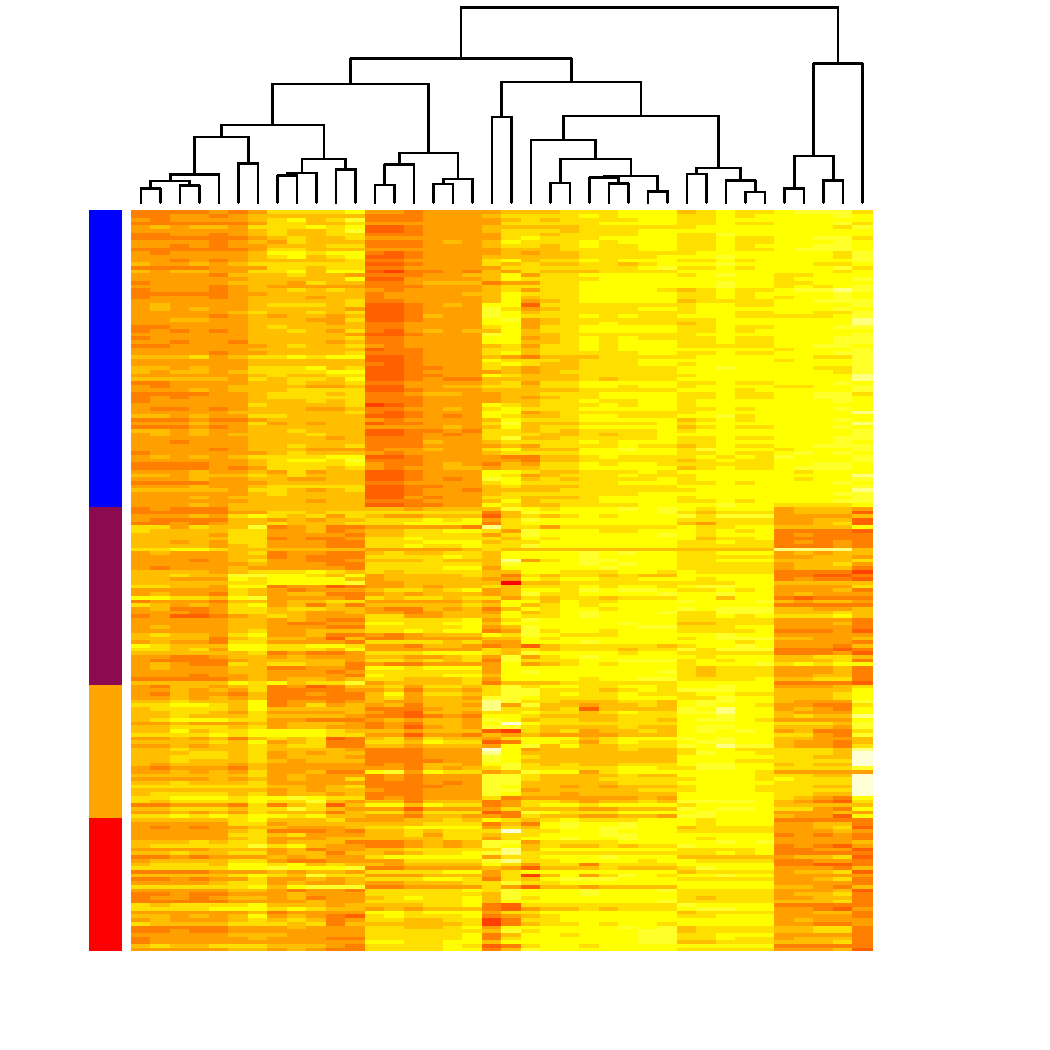
\includegraphics[width=\maxwidth]{figure/unnamed-chunk-51} 

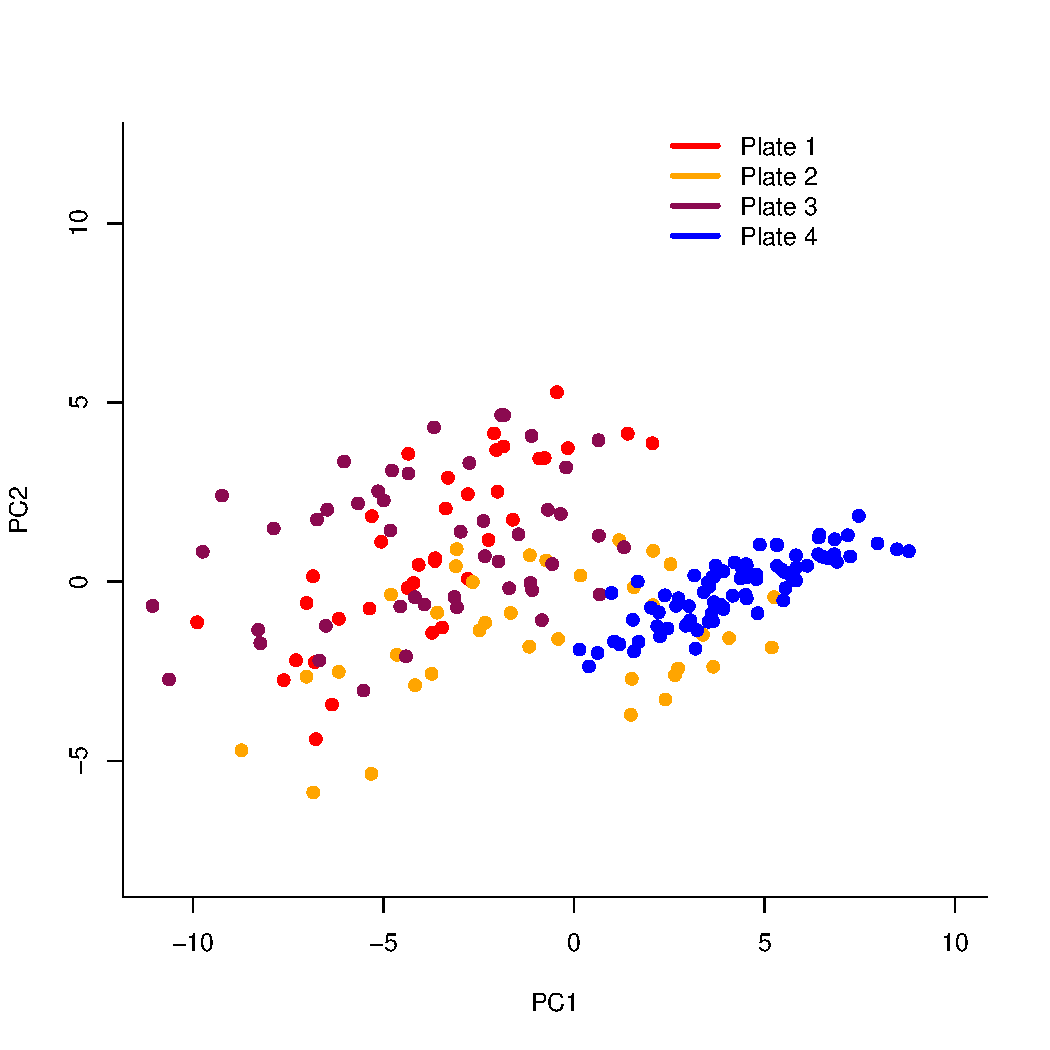
\includegraphics[width=\maxwidth]{figure/unnamed-chunk-52} 

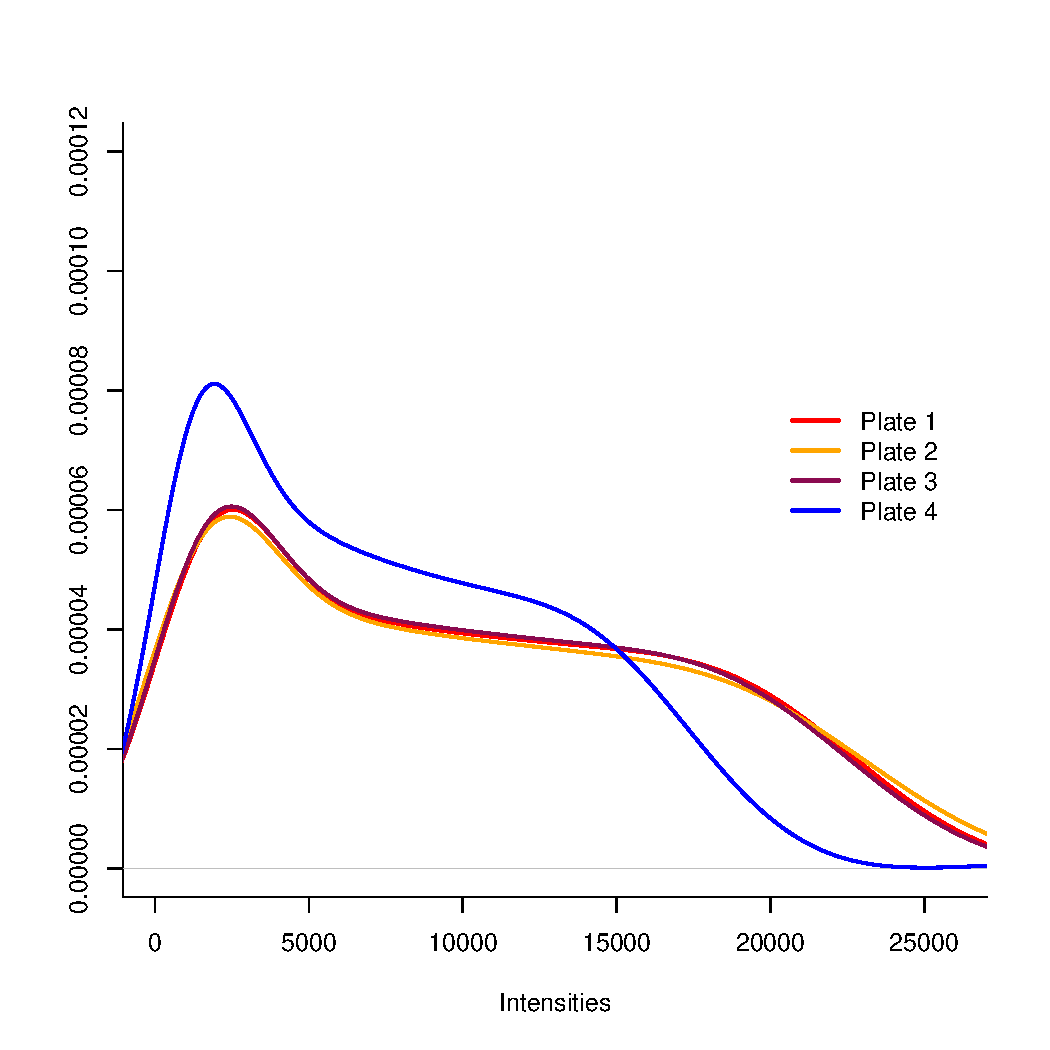
\includegraphics[width=\maxwidth]{figure/unnamed-chunk-53} 

\end{knitrout}

\subsubsection{Ontario-Blood}

\begin{knitrout}
\definecolor{shadecolor}{rgb}{0.969, 0.969, 0.969}\color{fgcolor}\begin{kframe}
\begin{alltt}
\hlkwd{source}\hlstd{(}\hlkwd{file.path}\hlstd{(funnormDir,} \hlstr{"paper_figures/generate.dis.val.roc.plots.R"}\hlstd{));}
\hlkwd{create.dis.val.roc.plots.blood}\hlstd{(}\hlkwc{print}\hlstd{=}\hlnum{TRUE}\hlstd{)}
\end{alltt}
\end{kframe}
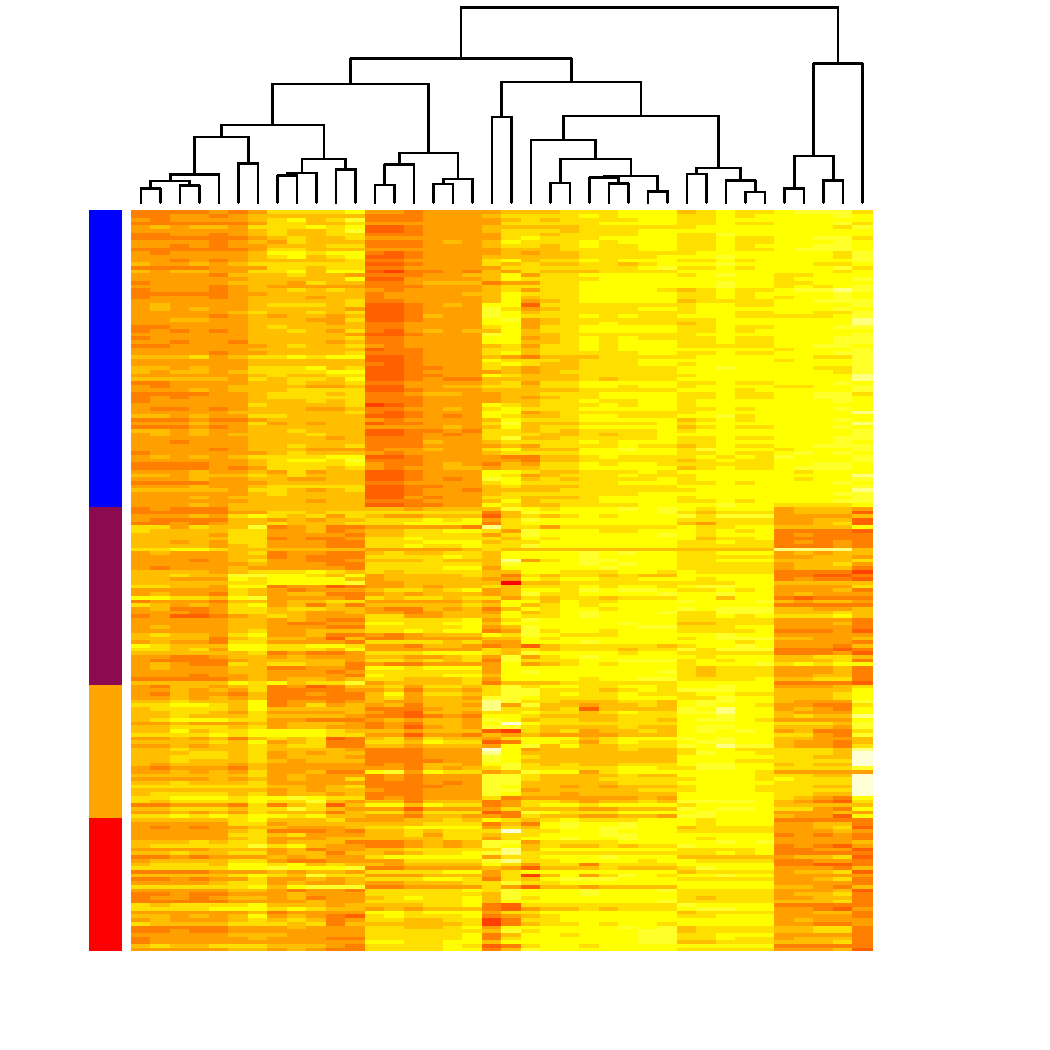
\includegraphics[width=\maxwidth]{figure/unnamed-chunk-61} 

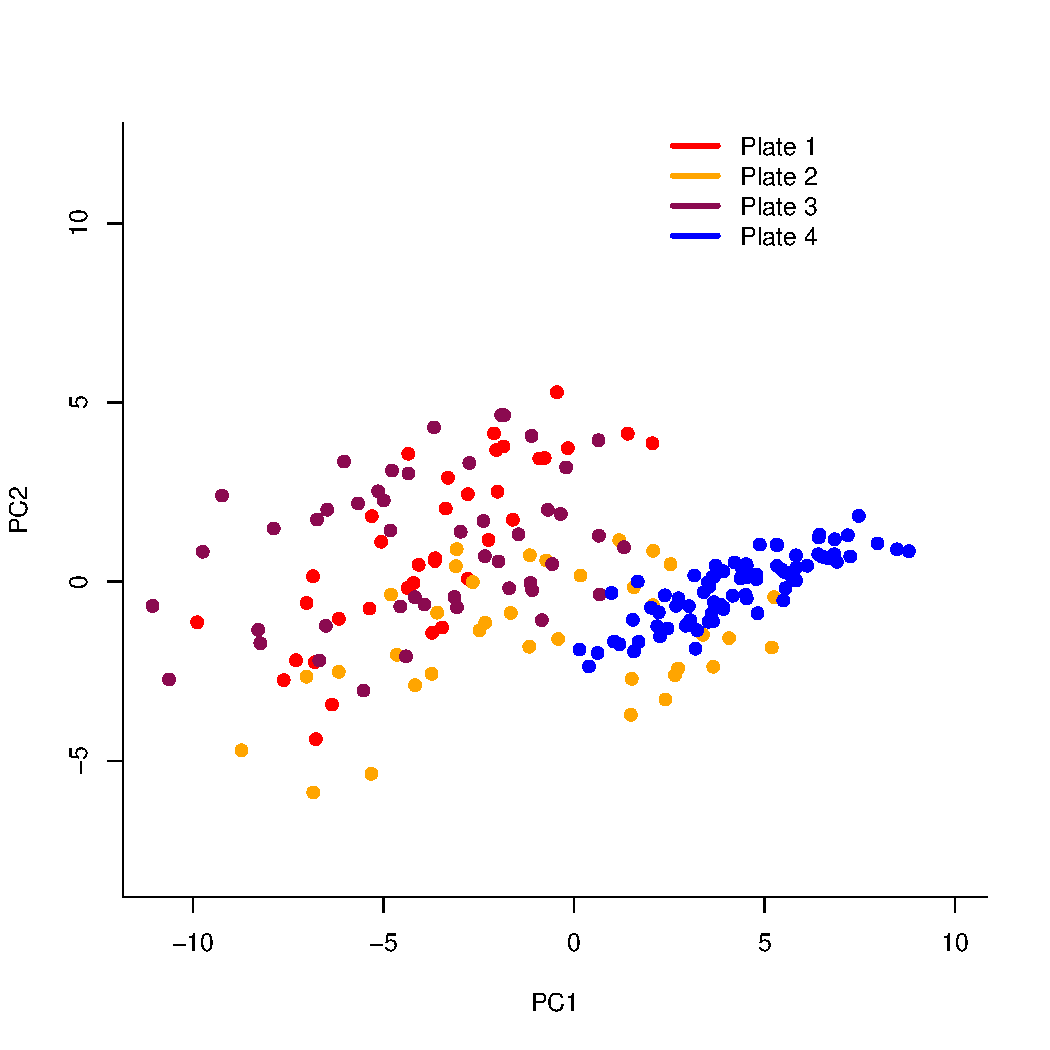
\includegraphics[width=\maxwidth]{figure/unnamed-chunk-62} 

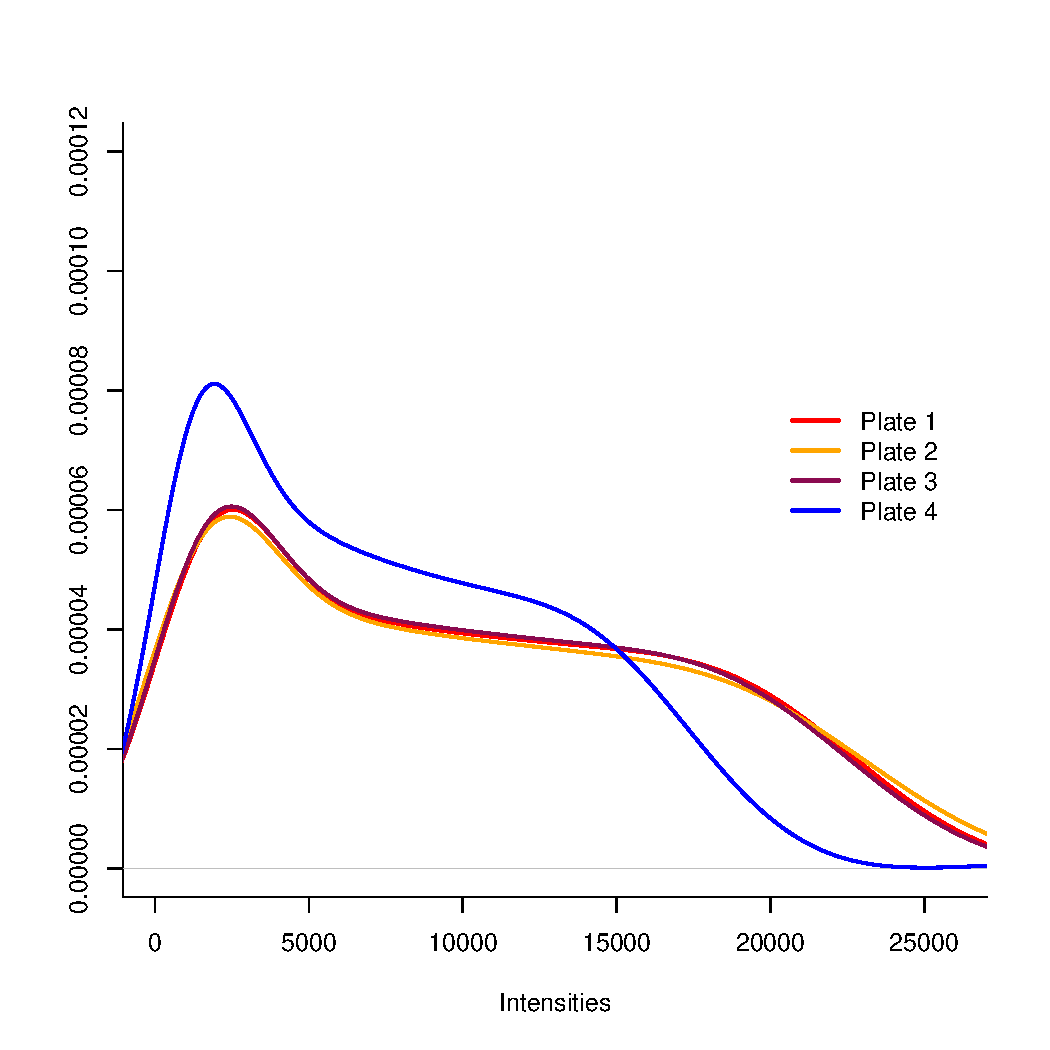
\includegraphics[width=\maxwidth]{figure/unnamed-chunk-63} 

\end{knitrout}

\subsubsection{KIRC}

\begin{knitrout}
\definecolor{shadecolor}{rgb}{0.969, 0.969, 0.969}\color{fgcolor}\begin{kframe}
\begin{alltt}
\hlkwd{source}\hlstd{(}\hlkwd{file.path}\hlstd{(funnormDir,} \hlstr{"paper_figures/generate.dis.val.roc.plots.R"}\hlstd{));}
\hlkwd{create.dis.val.roc.plots.kirc}\hlstd{(}\hlkwc{print}\hlstd{=}\hlnum{TRUE}\hlstd{)}
\end{alltt}
\end{kframe}
\includegraphics[width=\maxwidth]{figure/unnamed-chunk-71} 

\includegraphics[width=\maxwidth]{figure/unnamed-chunk-72} 

\includegraphics[width=\maxwidth]{figure/unnamed-chunk-73} 

\end{knitrout}


\subsection{Concordance curves}

\subsubsection{Ontario-EBV}

\begin{knitrout}
\definecolor{shadecolor}{rgb}{0.969, 0.969, 0.969}\color{fgcolor}\begin{kframe}
\begin{alltt}
\hlkwd{source}\hlstd{(}\hlkwd{file.path}\hlstd{(funnormDir,} \hlstr{"paper_figures/generate.concordance.plots.R"}\hlstd{));}
\hlkwd{create.overlap.plots.ebv}\hlstd{(}\hlkwc{print}\hlstd{=}\hlnum{TRUE}\hlstd{)}
\end{alltt}
\end{kframe}
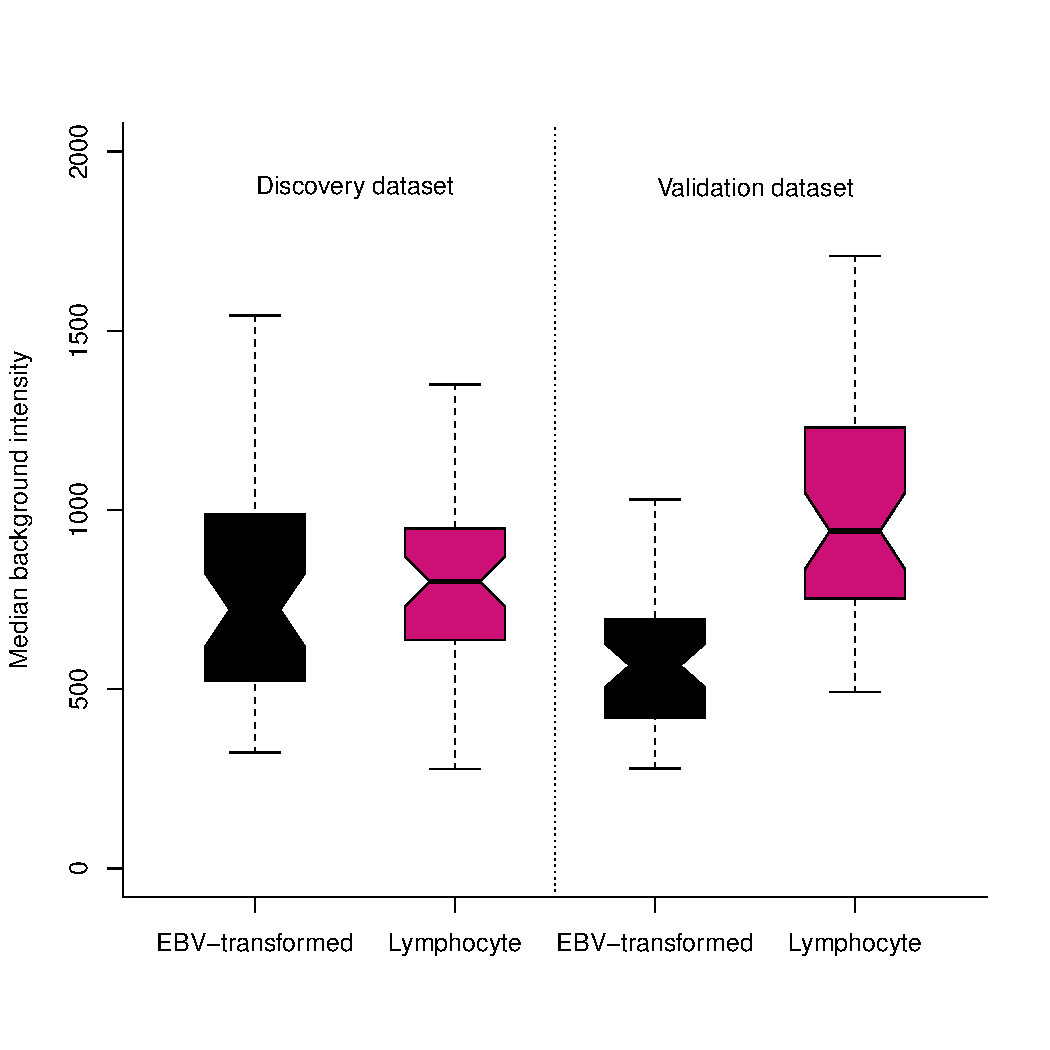
\includegraphics[width=\maxwidth]{figure/unnamed-chunk-81} 

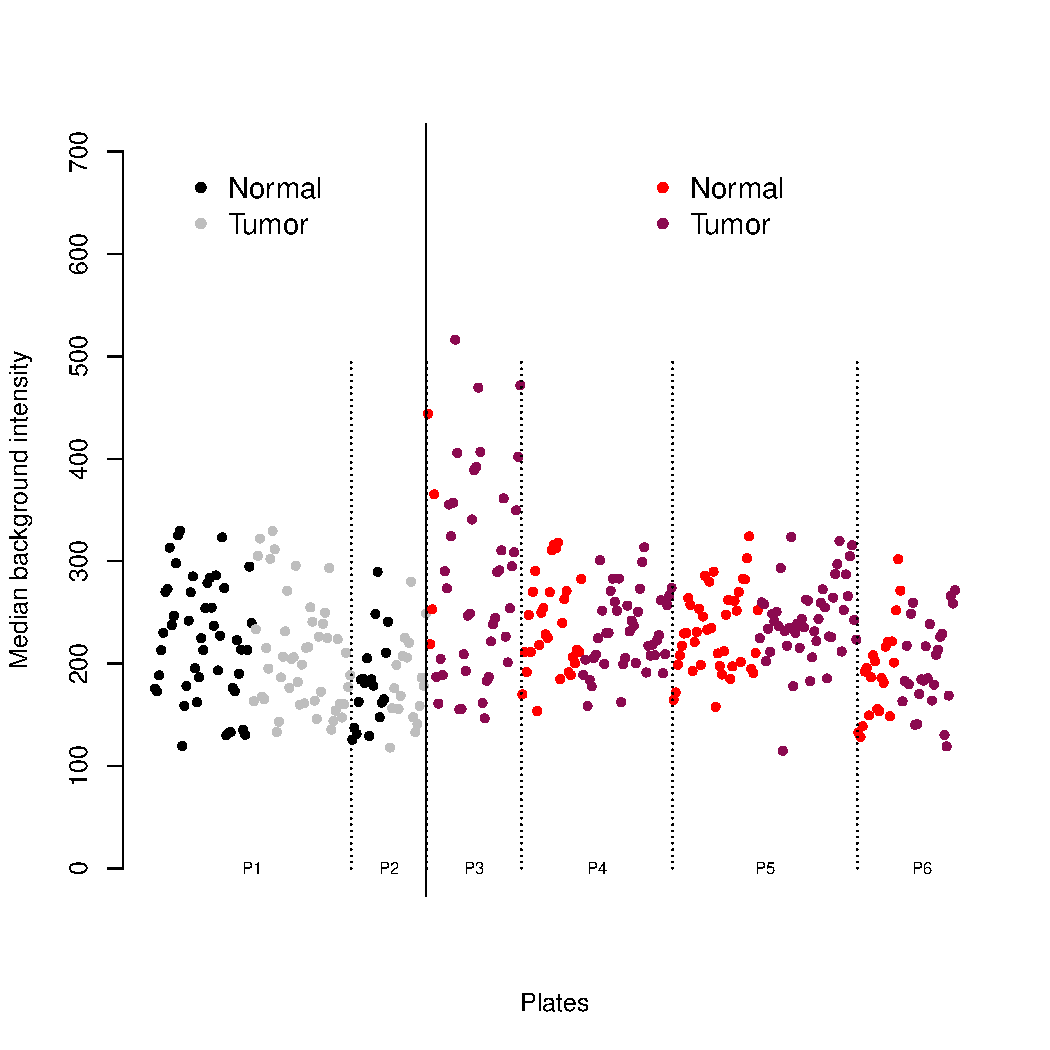
\includegraphics[width=\maxwidth]{figure/unnamed-chunk-82} 

\end{knitrout}

\subsubsection{KIRC}

\begin{knitrout}
\definecolor{shadecolor}{rgb}{0.969, 0.969, 0.969}\color{fgcolor}\begin{kframe}
\begin{alltt}
\hlkwd{source}\hlstd{(}\hlkwd{file.path}\hlstd{(funnormDir,} \hlstr{"paper_figures/generate.concordance.plots.R"}\hlstd{));}
\hlkwd{create.overlap.plots.kirc}\hlstd{(}\hlkwc{print}\hlstd{=}\hlnum{TRUE}\hlstd{)}
\end{alltt}
\begin{verbatim}
## NULL
\end{verbatim}
\end{kframe}
\end{knitrout}

\subsubsection{KIRC-27k}





